
\chapter{Analýza provisioning frameworků}

V~této kapitole rozeberu jednotlivé frameworky, pomocí kterých je možné nainstalovat operační systém. Jednou z~nutných podmínek je schopnost instalace operačních systémů CentOS a Debian. Ostatní operační systémy jsou výhoda, ale nejsou nezbytné. Kapitola též popisuje stroje, na kterých bude celý experiment testován spolu s~jejich konfigurací. Služby jsou konfigurovány tak, aby byly na oddělených virtuálních serverech a nemohly se vzájemně ovlivňovat. Na konci kapitoly vybereme framework Foreman z~důvodů níže uvedených.

\section{Metodika porovnání}

Než začnu zkoumání a hodnocení jednotlivých frameworků, je třeba si stanovit hodnotící kritéria, která mi umožní frameworky objektivně porovnávat a vybrat kandidáta pro kapitolu \b{Nasazení Foremanu}. Pokud to bude alespoň trochu možné, tak pro kritérium stanovím stupnici, na základě které bude možné frameworky mezi sebou porovnat.


Zhodnocení jednotlivých frameworků pro provisioning čistého hardwaru bylo provedeno jak z~pohledu kvality, tak i kvantity. Jakmile je framework nastaven a rozvržen, může být složité klientské servery zmigrovat z~jednoho na druhý. Kritéria zvolené při porovnáváni jsou následující:


\begin{itemize}
\item uzavřenost systému (licence),
\item dospělost projektu,
\item počet aktivních uživatelů,
\item složitost instalace frameworku,
\item stabilita,
\item složitost údržby,
\item hardwarová náročnost,
\item počet volitelných vlastností.
\end{itemize}

Následující podkapitoly přiblíží frameworky ke srovnání. Dále popíši jednotlivé parametry, podle kterých frameworky budeme porovnávat.



\section{Testovací laboratoř}


\subsection{Hardware}
\subsubsection{Master server}

Celý experiment byl testován na Intel x86 stroji se základní deskou X10SLM-F od výrobce SuperMicro. Na kartě je zapojen BMC modul pro vzdálené ovládání. Další fakta o~serveru jsou:

\begin{itemize}
\item Intel® Xeon® E3-1200 v3,
\item 16 GB RAM,
\item 1x 10Gbps Intel GE síťová karta,
\item 2x512 GB SSD disky zapojené jako JBOD. \footnote{Just a bunch of disks - v~překladu jen hromada disků}
\end{itemize}


\subsubsection{Instalovaný stroj}

Instalovaný stroj má tyto parametry:

\begin{itemize}
\item základní deska X10DDW-i,
\item Intel® Xeon® E3-1200 v3,
\item 16 GB RAM,
\item 1x 10Gbps Intel GE síťová karta,
\item 1x 1Gbps Intel XE síťová karta,
\item 1x 4TB HDD.
\end{itemize}

Koncept instalace serverů je navržen tak, že hlavní, tedy 10 Gbit síťová karta je zapojena do podsítě připojené do internetu. IP adresa na této síťové kartě přiřazena staticky na stroji. 1 Gbit port je zapojen do interní sítě oddělené od internetu, na které bude celý proces instalace probíhat. IP adresa je na tomto portu přiřazována pomocí DHCP. Připojení k~internetu při instalaci probíhá pomocí http-proxy, její adresa je zaslána serveru v~Kickstart/preseed konfiguračním souboru.


\subsubsection{Přepínač mezi stroji}

Jako přepínač mezi stroji byl využit Cisco SF550X-24. Na portu, na kterém je připojen master server, je povolen VLAN trunking. Pakety, které nejsou označkované (tagované), patří do VLAN 1. Na tomto portu jsou také povolené pakety otagované jako VLAN 222.

Na instalovaném stroji je konfigurace nasledující:

1Gbps síťová karta je připojena do VLAN 222 (trunkování VLAN není povoleno).
10Gbps síťová karta je připojena do VLAN 1 (trunkování VLAN není povoleno).

\subsection{Konfigurace strojů}

V~následujících podkapitolách popíši, jaká nastavení na serverech byla provedena.
\subsubsection{Master}

Na master stroji budeme všechny naše testované projekty mít v~kontejnerech. Přesněji řečeno to nebudou kontejnery, ale budeme využívat KVM (Kernel-based Virtual Machine) virtualizace, díky které můžeme jednotlivé části úplně oddělit od hypervisoru. Toto je míněho hlavně z~bezpečnostního hlediska. Jako operační systém, nad kterým budou jednotlivé služby spouštěny je vybrán Debian. Mezi důvodu patří nadstandardní stabilita, jedna z~největších komunit v~oblasti GNU/Linux a také velký výběr již vytvořených balíčků pro jakékoliv potřeby. Na síťovém portu jsou povoleny VLAN 1 a 222, přičemž pokud pokud ethernetový rámec tag s~informací o~VLANě neobsahuje, bude nastavena na 1. Tuto konfiguraci sítě pro operační systém Debian vidíme níže:

\begin{minted}{bash}
# /etc/network/interfaces
# interfaces(5) file used by ifup(8) and ifdown(8)
auto lo
iface lo inet loopback

auto br0
iface br0 inet dhcp
bridge_ports enp5s0
up /usr/sbin/brctl stp br0 off

auto enp5s0.222
iface enp5s0.222 inet static
        vlan-raw-device enp5s0

auto br1
iface br1 inet static
        address 192.168.4.4
        netmask 255.255.255.0
        bridge_ports enp5s0.222
        up /usr/sbin/brctl stp br1 on
\end{minted}

Jak vidíme výše, rozhraní br0 je VLAN 1 (dle nastavení na přepínači) a br1 je VLAN 222. Tato terminologie bude využívána i v~následujícím textu.


\section{Testované frameworky}

Kapitola níže popíše frameworky, které jsme k~naší analýze vybrali.
\section{Foreman}

Tento open source projekt spatřil světlo světa v~roce 2009, kdy byl založen programátory Ohadem Levym a Paulem Kellym. Foreman \cite{foreman} je komplexní nástroj pro správu celého životního cyklu jak hardhare strojů, tak těch virtuálních. Mezi hlavní části a funkce patří: provisioning, configurace serveru a poté jeho monitoring. Umožňuje automatizaci úkolů, které se opakují během prvotního nastavení infrastruktury. Dále Foreman nabízí správu konfigurací serverů, následovaných monitorováním a zobrazování trendů ze získaných dat.  Celý projekt je zaštítěn společností RedHat a jako jazyk byl vybrán Ruby on Rails. Databázi, do které budou ukládána data, si můžeme při instalaci vybrat -- patří mezi ně PostgreSQL, SQLite, MySQL a další. Foreman se dá také provozovat na jiných databázích, ovšem bez oficiální podpory.

Během provisioningu, Foreman z~velké části závisí na Smart Proxy, která je ve výchozím nastavení nainstalována na stejný server, jako Master uzel. Smart proxy hraje roli prostředníka v~kominikaci mezi Foremanem a externími službami. V~současnosi Smart Proxy obsahuje podporu pro služby: TFTP, DNS, DHCP, Puppet \& Puppet CA. Další služby je možné nainstalovat pomocí pluginů. Na obrázku \ref{arch-foreman} můžeme vidět komunikaci mezi Foremanem, Smart Proxy a službami.

\begin{figure}[h]\centering
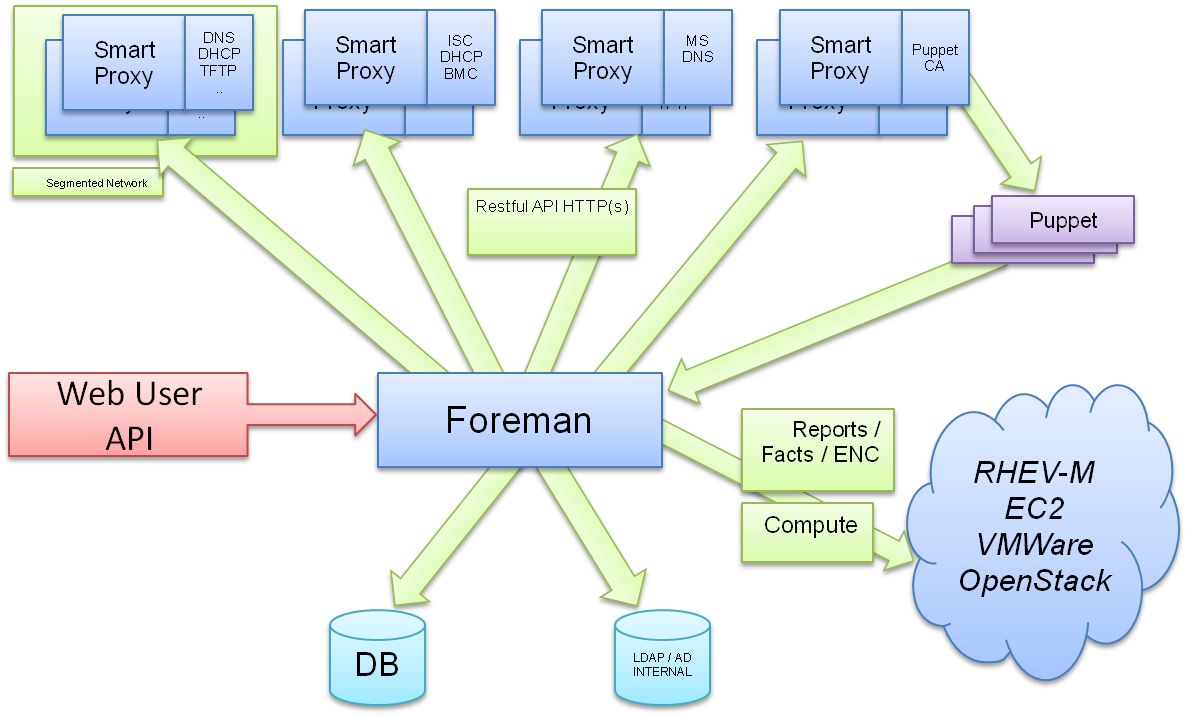
\includegraphics[width=0.8\textwidth]{files/foreman_architecture.png}
	\caption{Architektura Foremanu \cite{foreman-arch}}\label{arch-foreman}
\end{figure}


Provisioning serveru s~námi vybraným operačním systémem a požadovanou konfigurací je několika krokový proces. Prvně jě třeba vybrat operační systém s~přiřazeným instalačním médiem. Foreman již má několik operačních systémů založených na UNIXu v~sobě nakonfigurován a připraven přímo k~instalaci na stroje. Dalším krokem je vybrání rozdělení disků a šablony pro provisioning (pro příklad Kickstart nebo Preseed).

Když nainstalovaný server nabootuje pomocí PXE protokolu, vyšle broadcast zprávu pro DHCP server schopný přijímat DHCP žádosti. Smart Proxy pracující jako DHCP server odpoví a přidělí IP adresu novému hostu. PXE server je kontaktován a přesměruje nový stroj na TFTP server obsahující bootovací obraz disku. Nový stroj se pokusí o~získání obrazu, spustí ji a začne instalaci s~parametry, které byly obsažené v~šabloně ve Foremanu. Následovně, pokud je tak povoleno, proběhne jeden běh Puppetu. Foreman spoléhá na službě Puppet pro správu konfigurací a pro sbírání faktů o~serverech. Celý proces je zobrazen na obrázku \ref{foreman-arch-2}.

\begin{figure}[h]\centering
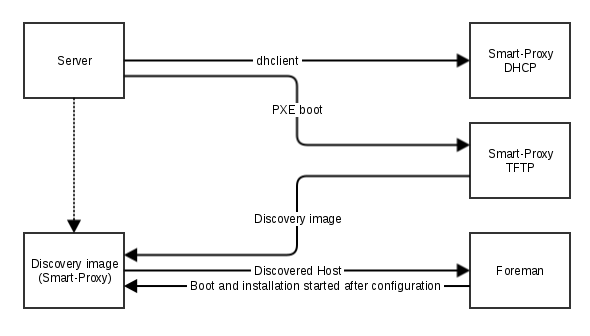
\includegraphics[width=0.8\textwidth]{files/discovery.png}
	\caption{Zavedení OS pomocí Foremanu \cite{foreman-arch2}}\label{foreman-arch-2}
\end{figure}


Foreman je schopen zavést široké spektrum operačních systémů založených na UNIXu. Mezi operační systémy, které se podle diskusních fór povedlo nainstalovat, patří: RHEL, Fedora, CentOS, Ubuntu, Debian, Solaris 8 and 10, OpenSUSE. Každopádně oficiální seznam operačních systémů, které Foreman podporuje, je poněkud kratší. Patří mezi ně: RHEL 6 and 7, CentOS 6 and 7, Fedora 19, Debian 7, Ubuntu 12.04 and 14.04 \cite{foreman-support-os}.

Foreman nabízí grafické rozhrací pro jednoduché využívání i méně schopnými uživateli. Je též dostupné RESTful API. Další variantou ovládání Foremanu je jeho nástroj pro ovládání z~příkazové řádky -- zvaný Hammer. Pomocí něj je možné jednotlivé dílčí kroky skriptovat. Foreman je jednoduše rozšiřitelný pomocí Rails Engines. To ukazuje široká škála již dostupných rozšíření. Mezi ně patří například rozšíření Azure, Digital Ocean a další - pro přímý provisioning virtuálních serverů ve zmíněných cloudech.

\subsection{Foreman Smart Proxy}

Jádrem řídícího systému Foremanu pro vzdálené části infrastruktury jsou Smart Proxy \cite{foreman-proxy}, což jsou malé a modulární aplikace vytvořené v~Ruby. Zjednodušeně, pokud něco spravovat, spustíme jednu z~těchto ruby aplikací v~místě, kde potřebujeme. Například, místo toho, abychom se manuálně připojili k~DHCP serveru, podívali se na zápůjčky IP adres, přímo se pomocí REST API DHCP serveru zeptáme na volnou IP adresu, kterou nám DHCP server vrátí. Kód těchto proxy serverů je cíleně velmi krátký -- okolo 1000 řádků, díky čemuž není tak těžké jednotlivým částem porozumět a dopsat libovolný modul.

Mezi tyto smart proxy moduly patří:
\begin{itemize}

\item DHCP, DNS, TFTP,
\item BMC/IPMI,
\item Puppet, Puppet CA,
\item MCollective \cite{mcollective}.
\end{itemize}

Foreman obsahuje koncept zvaný Compute Resources. Tento nápad cílí na provisioning virtuálních serverů (také bare metal) na veřejných a soukromých cloudech. Podporuje tedy například VMWare infrastrukturu, nebo EC2.

% Stroje ve Foremanu jsou děleny na dvě části -  managed a unmanaged. Managed stroje můžeme například restartovat, nainstalovat nový OS, atp. Unmanaged stroj je zjednodušeně jen Puppet slave (v puppet terminologii Agent), který komunikuje s naším Puppet Masterem. Unmanaged server je možné přeměnit na managed a následně ho přes grafické rozhraní ovládat. Je tedy možné do nástroje přidat ve velkém až stovky serverů, které už fungují.

% Pokud chceme vytvořit nový host (tj. provision host), ať už na bare metalu, nebo na cloudu, vybereme, kam instalovat. Pokud je stroj bare metal, námi vytvořený host a fyzický stroj v datacetru se mezi sebou matchují pomocí mac adresy.

% Provisioning Templates


% Integrace puppetu.

% Puppet je velmi silně integrován do foremanu.

\section{Razor}

Razor \cite{razor} je jednou z~aplikací pro zavedení operačního systému na bare-metal servery a virtuální systémy. Jedním z~cílů frameworku je dostání serveru do stavu, kdy aplikace pro zaslání konfgurací na server (jako jsou např. Ansible nebo Puppet) mohou převzít kontrolu.

Servery nově přidané do Razoru pomocí PXE standadu stáhnou a spustí obraz disku zvaný Razor microkernel image, který aplikaci zašle informace o~serveru a vyčká na další instrukce. Razor podle předem předpřipravených pravidel od uživatele vyhodnotí, jaký model (tj. jaký operační systém, jaké diskové rozložení, atp.) má na server aplikovat. Nový uzel začne následovat instrukce dle modelu, odpovídá Razoru a dokončí instalaci. Model může obsahovat např. instalaci Puppetu a registraci k~nějakému serveru s~běžící aplikací pro správu serverů.

\section{Stacki}

Stacki \cite{stacki} je nabízen ve dvou základních plánech. V~plánu zdarma, ten ale nenabízí webové rozhraní. Placený plán sice přes webovou stránku ovládat lze, skrývá ale v~sobě jiná omezení. Mezi tato omezení paří například nemožnost instalace distribucí založených na Debianu (tedy i Ubuntu, které je jedním z~našich požadavků), dále neobsahuje podporu pro UEFI. UEFI v~nasěm případě problém není, protože SuperMicro základní karty v~nastavení umožňují změnu na Legacy Boot (BIOS), absence podbory Debian distribucí je ale pro nás závážná, až klíčová.

\subsection{Edice zdarma}

Základní verzi Stacki můžeme nalézt zdarma, bohužel je ořezaná o~určité vlastnosti. Jednou z~možností je stažení rpm balíčku pro CentOS. Po instalaci balíčku dostaneme skript, který server přetransformuje na Stacki frontend. Druhou možností je, stejně jako u~placené verze, připraný ISO obraz pro instalaci na stroj bez operačního systému.

\subsection{Pro plán}

Placená edice Stacki softwaru je nabízena ve 14-ti denní zkušební verzi, tu jsem také pro tento experiment použil. Po registraci na webu produktu je odeslán e-mail s~odkazem na stažení iso souboru. Obraz je ve své podstatě CentOS linux (můžeme si vybrat CentOS 6, či 7) přípravený pro vypálení na CD, nebo zkopírování na USB disk pro následovné zavedení systému a instalaci na čistý stroj. Tento postup je odlišný od ostatní opensource konkurence, jež nabízejí svoje provision frameworky většinou jako balíčky pro linuxové disribuce. Cena placené edice je 100 USD/rok na jeden uzel, hlavní výhodou je již zmíněná podpora UEFI a možnost instalace Ubuntu a v~neposlední řadě placená podpora.



\section{OpenStack Ironic}

OpenStack \cite{openstack} je škálovatelná, open-source platforma pro stavbu veřejných či privátních cloudů. Jako distribuční model převažuje IaaS, česky přeloženo jako \uv{Infrastruktura jako služba}. V~takovémto modelu se poskytovatel služeb zavazje poskytnout infrastrukturu -- ať už virtualizované, tak i hardware servery. Příklady komerčních IaaS jsou např. Amazon Web Services, nebo Microsoft Azure.  OpenStack je stavěný na velké výpočetní, datové i síťové zdroje v~datacentrech, u~čehož je vě ovládáno přes webové rozhraní.

Všechny OpenStack služby mezi sebou komunikují na bázi RESTful API, k~tomuto využívají HTTP protokol pro výměnu informací a dat. Jednou komponentou je právě Ironic pro instalaci bare metal serverů.

OpenStack je orientován na obrovské clustery. Věřím, že v~určitých případech může být správnou volbou i pro provisioning, v~našem případě ale taková volba připadá jako kolos. Už jen instalace celého frameforku na jeden systém (v~mém případě vybraném DevStacku) trvala něco přes půl hodinu. Z~důvodů nevhodnosti pro naše využití jsem se s~testováním tohoto frameworku dále nezabýval.


\section{Spacewalk}


Spacewalk \cite{spacewalk} je open source nástrojem pro administraci Linux serverů. Licencí, pod kterou je distribuován, je GPLv2\cite{gpl2}. Spacewalk je software řízený komunitou, vyvinuly se z~něj ale i nějaké komerční produkty -- mezi ně patří například Red Hat Satellite \cite{satellite} nebo Novell SUSE Manager \cite{suse-manager}. Vývoje framerworku Spacewalk začal v~červnu 2008 a v~té době se oficiálně stal open-source projektem. Základem je Red Hat Network, založený v~roce 2001 -- z~tohoto projetu se později stal oddělený Red Hat Satellite produkt.

Spacewalk má mnoho vlastností umožňujících linuxovým administrátorům správu hardwaru. Umožňuje instalovat a aktualizovat systémy, konfigurovat systémy ve skupinách, zavést operační systém na bare-metal server a následně ho nastavit, včetně instalace monitorování. Spacewalk též spolupracuje s~virtualizačními platformami, jako jsou VMWare, nebo Xen \cite{xen}, na kterých vytvoří virtuální servery. Administrační software podporuje mnoho linuxových distribucé, mezi které patří např. Fedora, CentOS, SLES and Debian na architekturách 32bit, i 64bit.


\subsection{Licence}

V~této práci se budu zabývat pouze open-source frameworky, tedy pokud nějaký framework chceme zvažovat, musíme nejdříve zjistit, zda nám to licence projektu dovoluje. Licence frameworku může ovlivnit licenci díla, kde framework použijeme (tedy i tuto bakalářskou práci). Důvody pro open-source jsou zřejmé:

\item nulové počáteční náklady - získáme zdarma produkt, krerý by jinak společnost vyvíjela několik měsíců. Díky tomu je ušetřeno na počátečních nákladech,
\item bezpečnost - oprava 0 Day \cite{0day} zranitelností a dalších chyb je díky komunitě skoro okamžítá,
\item žádné proprietární uzamčení a lepší kvalita kódu.

Licence se dají rozdělit podle stupně přísnosti. Níže uvedené rozdělení je od nejméně přísného až po nejstriktnější:

\begin{itemize}
\item Public Domain,
\item permisivní,
\item LGPL,
\item copyleft,
\item AGPL.
\end{itemize}

Všechny analyzované frameworky se nacházejí pod určitou open-source licencí, nebo alespoň mají ekvivalentní open-source edici. OpenStack Ironic, Foreman, Cobbler i MaaS jsou kompletně open-source a zdarma.


\begin{table}[h]
\centering
\caption{Frameworky: License}
\label{Frameworky_licence}
\begin{tabular}{lllllll}
\toprule
 Foreman & Ironic & Razor & Stacki & Spacewalk & Cobbler \\ \midrule
 GNU GPL 3    &  Apache &  Apache &  BSD, placená   &   GNU GPL 2  & GNU GPL 2
\end{tabular}
\end{table}




\subsection{Stáří projektu}

\uv{Nedospělý}, či netestovaný kód, který se může jednoduše rozbít, přímo koreluje se stářím frameworku. Je proto důležité se ujistit, že projekt, který vybereme bude použitelný a dospělý.  V~naší analýze je dospělost spočítána pomocí počtu let, jak dlouho je framework vyvíjen.

Počet uživatelů či počet nasazení systému nám může ukázat určité náznaky, jako jaká je populárnost systému u~určité společnosti a které důvody se za tím skrývají. Tato hodnota, aby byla přesná, není jednoduše zjistitelná. Určité metriky jsou ale veřejně dostupné -- mezi ty patří například počet forků na GitHubu, počet uživatelů v~mailing listu, počet velkých firem, které se rozhodly pro nasazení frameworku (zde vycházím z~předpokladu, že ve velké společnosti tým na takový úkol bude mít větší počet pracovníků a tím i přispěvatelů do projektu). Tyto hodnoty nám můžou nastínit určitý odhad, kolik nasazení bylo. Toto nám také v~určité míře ukazuje, jaká rychlost bude při opravách různých chyb, či rychlost přidávání dalších funkcí.



\begin{table}[h]
\centering
\caption{Frameworky: Stáří projektu}
\label{Frameworky_oldness}
\begin{tabular}{lllllll}
\toprule

 Foreman & Ironic & Razor & Stacki & Spacewalk & Cobbler \\ \midrule
  2009        & 2013       &  2013     & 2015       &  2008         & 2011
\end{tabular}
\end{table}

\begin{table}[h]
\centering
\caption{Frameworky: počet forků na GitHubu}
\label{Frameworky_oldness}
\begin{tabular}{lllllll}
\toprule

 Foreman & Ironic & Razor & Stacki & Spacewalk & Cobbler \\ \midrule
  598        & 188       &  139     & 25       &  127         & 402
\end{tabular}
\end{table}


%
% \subsection{Složitost instalace}
%
% Dalších z hlavních bodů, které musíme při výběru frameworku zvažovat, je složitost instalace takovéhoto systému pro provizi serverů. Jedním
%
% \subsection{Stabilita}
%

\subsection{Složitost užití}

Všechny analyzované frameworky mají webové grafické rozhraní, pomocí kterého je možné servery provizovat. Díky tomu by měla být uživatelská přívětivost na slušné úrovni. Výjimkou je Razor, u~kterého je grafické rozhraní pouze placené verzi (tj. Puppet Enterprise). Objevil jsem grafické rozhraní \cite{puppet-dashboard}, které by zmíněný problém mělo vyřešit, není ale součástí analýzy.

\subsection{HW požadavky}

Dříve, než začneme instalovat jakýkoliv software, musíme se ujistit, zda hadware, na který program chceme nainstalovat, je dostatečný. I~přes to, že hardware dostupný pro experiment se zdál dostatečný, v~případě instalace Ironic nestačil. Pro jeho provozování je třeba sestavit celý cluster -- pro experiment tedy místo OpenStacku byl vybrán DevStack \cite{devstack}, který bohužel svojí rychlostí neoslnil. Všechny ostatní frameworky s~poskytnutým výpočetním výkonem a pamětí problém neměly.


\subsection{Podpora discovery}

Je důležité, aby vybraný framework podporoval tzv. discovery -- tedy objevení a zjištění základních informací o~serverech, které které jsou nové a ještě v~databázi nejsou. Většina frameworků má tuto funkcionalitu vytvořenou způsobem linuxové image, která se načte místo operačního systému na neznámých strojích. Tento malý linux si poté pokusí nastavit připojení k~síti, DNS, a pokud se zdaří, odešle frameworku zpět informace o~novém serveru. Mezi informace může patřit například počet procesorů, velikost paměti, nebo typ síťové karty. Ve frameworku Foreman se tato funkcionalita nazývá Discovery \cite{foreman-discovery}, v~Razoru zase EL Microkernel \cite{el-microkernel}. Tabulka \ref{Frameworky_discovery} ukazuje, zda testovaný nástroj objevování nových strojů podporuje.



\begin{table}[h]
\centering
\caption{Frameworky: Podpora funkcionality discovery}
\label{Frameworky_discovery}
\begin{tabular}{lllllll}
\toprule

- & Foreman & Ironic & Razor & Stacki & Spacewalk & Cobbler \\ \midrule
  & ANO        &  ANO      &  ANO     & ANO       &  ANO         & NE
\end{tabular}
\end{table}


\subsection{Podpora operačních systémů}

Jedním z~prvních požadavků bylo, že daný framework bude podporovat instalaci různých operačních systémů (alespoň linuxových distribucí). Například MaaS podporuje pouze Ubuntu -- je vydáván společností Canonical (společnost zaštitující Ubuntu). Proto mnoho funkcionalit MaaS je již zakomponováno do Ubuntu. Cobbler i Ironic mají podporu instalace pouze linuxových distribucí. Foreman zvládne jak různé linuxové distrubuce, tak BSD systémy, i Windows. Podporu Windows s~určitými úravami má také Razor. Framework Stacki je stavěn předně pro linuxovou distribuci CentOS (v~oficiální podpoře), Debian a Ubuntu pouze s~komunitní podporou. V~tabulce \ref{Frameworky_os} jsou vidět frameworky a jejich podporu instalovaných operačních systémů:



\begin{table}[h]
\centering
\caption{Frameworky: Podpora operačních systémů}
\label{Frameworky_os}
\begin{tabular}{lllllll}
\toprule

 Foreman & Ironic & Razor & Stacki & Spacewalk & Cobbler \\ \midrule
 Linux        & Linux       & Linux      & Linux       & Linux          & Linux \\
 Windows         &        & Windows      &        &           &

\end{tabular}
\end{table}




\section{Závěr}


V~této kapitole popíši a shrnu jednotlvé frameworky v~jejich silných i slabých bodech podle poznatků, které jsem získal při testování systémů a podle posbíraných statistických dat.


\subsection{Foreman}



Z~výše testovaných frameworků po analýze byl vybrán Foreman. Hlavní výhodou bylo jeho grafické rozhraní, pomocí kterého může administrátor vykonat reinstalaci serveru na jakémkoliv zařízení s~webovým prohlížečem. To samé se týká i serverového technika, který je schopen práci vykonat na svém telefonu, stojící vedle serveru v~serverovně. Jeho instalace byla v~porovnání s~ostatními frameworky stejně obtížná, z~důvodu, že implicitní konfigurace není ideální a je třeba systém hluboce nastudovat, pokud ho nevyužíváte na uživatelské úrovni. Výhodou jsou již vytvořené balíčky pro master server, Smart Proxy, i nějaké pluginy do operačního systému Debian, což konkurence v~podobě Spacewalk, Stacki a dalších nenabízí. Mezi další důvody mého výběru Foremanu patří jedna z~největších komunit v~této oblasti a také časté vydávání nových verzí. Nasazením frameworku se věnuje příští kapitola.


\subsection{Ostatní frameworky}


V~této části práce následuje přehledná tabulka popisující, jak si frameworky v~jednotivých kategoriích vedly. Podrobnější tabulky o~každém kritériu byly uvedeny v~příslušných sekcích.
\newpage
\begin{table}[H]
\centering
\caption{Srovnání frameworků}
\label{srovnani-frameworku}
\rotatebox{90}{

\begin{tabular}{@{}l|llllll@{}}
\toprule

metrika &	Foreman & Ironic & Razor & Stacki & Spacewalk & Cobbler  \\ \midrule
Uzavřenost systému &  GNU GPL 3    &  Apache &  Apache &  BSD, placená   &   GNU GPL 2  & GNU GPL 2 \\
Dospělost projektu &   2009        & 2013       &  2013     & 2015       &  2008         & 2011 \\
Počet forků na GitHubu & 598        & 188       &  139     & 25       &  127         & 402 \\
Intalované OS & Linux        & Linux       & Linux      & Linux       & Linux          & Linux \\
& Windows         &        & Windows      &        &           & \\
Podpora discovery & ANO        &  ANO      &  ANO     & ANO       &  ANO         & NE \\
%Počet aktivních uživatelů & & & & & & \\
% Složitost instalace frameworku & & & & &  & \\
% Stabilita & & & & &  & \\
% Složitost údržby & & & & & &  \\
% Podpora discovery  & & & & &  & \\
% Hardwarová náročnost & & & & &  & \\
% Počet features & & & & &  & \\ \bottomrule
\end{tabular}
}
\end{table}

\begin{table}[h]
\centering
\caption{Informace o~frameworcích}
\label{my-label}
\begin{tabular}{@{}lll@{}}
\toprule

Framework &	Webová stránka &	Testovaná verze  \\ \midrule
Foreman & https://www.theforeman.org/ & 1.14.3 \\
Ironic & https://wiki.openstack.org/wiki/Ironic & 1:5.1.2-0ubuntu1  \\
Razor & https://github.com/puppetlabs/razor-server & 1.7.0 \\
Stacki & https://github.com/StackIQ/stacki & 4.0  \\
Spacewalk & https://spacewalk.redhat.com/ &  2.6 \\
Cobbler & http://cobbler.github.io/ & 2.8.0  \\  \bottomrule
\end{tabular}
\end{table}
\newpage

Tabulka výše ukazuje verze frameworků testované v~této analýze spolu s~odkazy na domácí stránky projektů.
